% ============================================================================
%  fig_rtl.tex - Jerarquía RTL del núcleo (pong_top) con sus señales
%  Pong en FPGA - Electrónica Digital 1 - UNAL
%  Juan David Ortiz Muñoz, David Eduardo Chivata Arias, Daniel Felipe Castro González
%  Compilar con: pdflatex fig_rtl.tex
% ============================================================================
\documentclass[border=6pt]{standalone}
\usepackage[utf8]{inputenc}
\usepackage[T1]{fontenc}
\usepackage{lmodern}
\usepackage{tikz}
\usetikzlibrary{positioning,arrows.meta,calc,fit,backgrounds}
\begin{document}
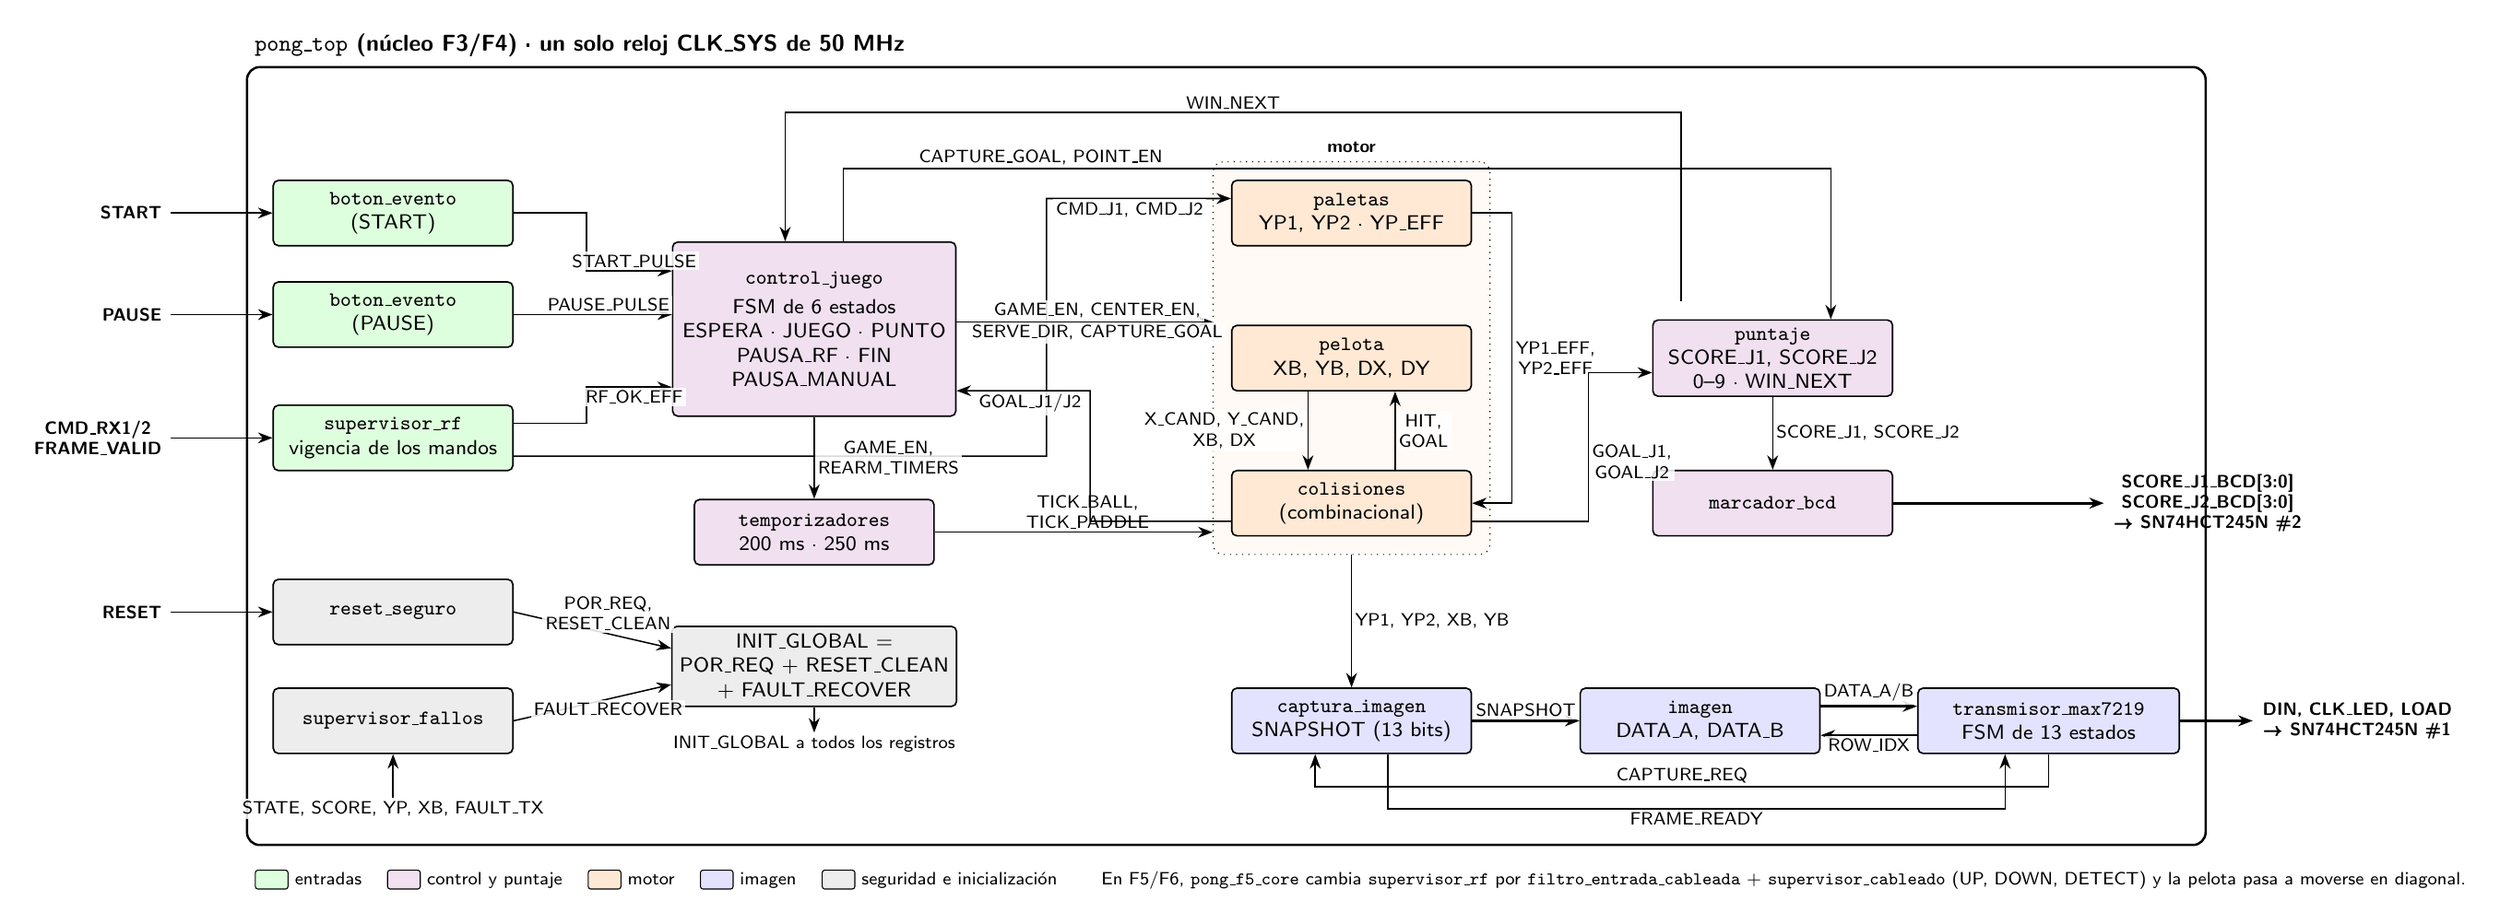
\begin{tikzpicture}[
    font=\sffamily\footnotesize,
    >={Stealth[length=2mm]},
    mod/.style={draw, rounded corners=2pt, align=center, minimum width=3.3cm, minimum height=0.9cm, inner sep=3pt, line width=0.6pt},
    ent/.style={mod, fill=green!13},
    ctl/.style={mod, fill=violet!12},
    mot/.style={mod, fill=orange!17},
    vid/.style={mod, fill=blue!11},
    seg/.style={mod, fill=gray!14},
    pin/.style={font=\sffamily\scriptsize\bfseries, align=center},
    sig/.style={->, line width=0.55pt},
    bus/.style={->, line width=1.2pt},
    lbl/.style={font=\sffamily\scriptsize, align=center, inner sep=1.2pt, fill=white, fill opacity=0.85, text opacity=1},
]

% ------------------------------------------------------------- Columna de entradas
\node[ent] (start) at (0, 7.4) {\texttt{boton\_evento}\\(START)};
\node[ent] (pause) at (0, 6.0) {\texttt{boton\_evento}\\(PAUSE)};
\node[ent] (rf)    at (0, 4.3) {\texttt{supervisor\_rf}\\vigencia de los mandos};
\node[seg] (rst)   at (0, 1.9) {\texttt{reset\_seguro}};
\node[seg] (flt)   at (0, 0.4) {\texttt{supervisor\_fallos}};

% ------------------------------------------------------------- Control
\node[ctl, minimum height=2.4cm, minimum width=3.9cm] (fsm) at (5.8, 5.8) {\texttt{control\_juego}\\[2pt]FSM de 6 estados\\ESPERA · JUEGO · PUNTO\\PAUSA\_RF · FIN\\PAUSA\_MANUAL};
\node[ctl] (tmr) at (5.8, 3.0) {\texttt{temporizadores}\\200 ms · 250 ms};
\node[seg, minimum width=3.9cm] (init) at (5.8, 1.15) {INIT\_GLOBAL =\\POR\_REQ + RESET\_CLEAN\\+ FAULT\_RECOVER};

% ------------------------------------------------------------- Motor
\node[mot] (pal) at (13.2, 7.4) {\texttt{paletas}\\YP1, YP2 · YP\_EFF};
\node[mot] (pel) at (13.2, 5.4) {\texttt{pelota}\\XB, YB, DX, DY};
\node[mot] (col) at (13.2, 3.4) {\texttt{colisiones}\\(combinacional)};
\begin{scope}[on background layer]
  \node[draw, dotted, rounded corners, fill=orange!4, inner sep=7pt, fit=(pal)(col),
        label={[font=\sffamily\scriptsize\bfseries, anchor=south]north:motor}] (motor) {};
\end{scope}

% ------------------------------------------------------------- Puntaje
\node[ctl] (pun) at (19.0, 5.4) {\texttt{puntaje}\\SCORE\_J1, SCORE\_J2\\0–9 · WIN\_NEXT};
\node[ctl] (bcd) at (19.0, 3.4) {\texttt{marcador\_bcd}};

% ------------------------------------------------------------- Imagen
\node[vid] (cap) at (13.2, 0.4) {\texttt{captura\_imagen}\\SNAPSHOT (13 bits)};
\node[vid] (img) at (18.0, 0.4) {\texttt{imagen}\\DATA\_A, DATA\_B};
\node[vid, minimum width=3.6cm] (tx) at (22.8, 0.4) {\texttt{transmisor\_max7219}\\FSM de 13 estados};

% ------------------------------------------------------------- Caja pong_top
\begin{scope}[on background layer]
  \node[draw, line width=0.9pt, rounded corners=5pt, inner sep=10pt, fit={(start)(flt)(tx)(pun)(pal)($(pal.north)+(0,1.2)$)($(tx.south)+(0,-0.9)$)},
        label={[font=\sffamily\small\bfseries, anchor=south west]north west:\texttt{pong\_top} (núcleo F3/F4) · un solo reloj CLK\_SYS de 50 MHz}] (top) {};
\end{scope}

% ------------------------------------------------------------- Pines de entrada
\draw[sig] ($(start.west)+(-1.4,0)$) node[pin, left] {START} -- (start.west);
\draw[sig] ($(pause.west)+(-1.4,0)$) node[pin, left] {PAUSE} -- (pause.west);
\draw[sig] ($(rf.west)+(-1.4,0)$) node[pin, left] {CMD\_RX1/2\\FRAME\_VALID} -- (rf.west);
\draw[sig] ($(rst.west)+(-1.4,0)$) node[pin, left] {RESET} -- (rst.west);

% ------------------------------------------------------------- Entradas -> control
\draw[sig] (start.east) -- ++(1.0,0) |- node[lbl, pos=0.78, above] {START\_PULSE} ([yshift=8mm]fsm.west);
\draw[sig] (pause.east) -- node[lbl, above, pos=0.6] {PAUSE\_PULSE} (pause.east -| fsm.west);
\draw[sig] ([yshift=2mm]rf.east) -- ++(1.0,0) |- node[lbl, pos=0.78, below] {RF\_OK\_EFF} ([yshift=-8mm]fsm.west);
\draw[sig] ([yshift=-2.5mm]rf.east) -- (9.0, 4.05) -- (9.0, 7.6) -- node[lbl, below, pos=0.45] {CMD\_J1, CMD\_J2} ([yshift=2mm]pal.west);

% ------------------------------------------------------------- Inicialización
\draw[sig] (rst.east) -- node[lbl, above, pos=0.6] {POR\_REQ,\\RESET\_CLEAN} ([yshift=2.5mm]init.west);
\draw[sig] (flt.east) -- node[lbl, below, pos=0.6] {FAULT\_RECOVER} ([yshift=-2.5mm]init.west);
\draw[sig] (init.south) -- ++(0,-0.35) node[lbl, below, align=center] {INIT\_GLOBAL a todos los registros};
\draw[sig] ($(flt.south)+(0,-0.6)$) node[lbl, below] {STATE, SCORE, YP, XB, FAULT\_TX} -- (flt.south);

% ------------------------------------------------------------- Control -> temporizadores y motor
\draw[sig] (fsm) -- node[lbl, right] {GAME\_EN,\\REARM\_TIMERS} (tmr);
\draw[sig] ([yshift=1mm]fsm.east) -- node[lbl, above, pos=0.55] {GAME\_EN, CENTER\_EN,} node[lbl, below, pos=0.55] {SERVE\_DIR, CAPTURE\_GOAL} ([yshift=1mm]fsm.east -| motor.west);
\draw[sig] (tmr.east) -- node[lbl, above, pos=0.55] {TICK\_BALL,\\TICK\_PADDLE} (tmr.east -| motor.west);

% ------------------------------------------------------------- Dentro del motor
\draw[sig] ([xshift=-6mm]pel.south) -- node[lbl, left] {X\_CAND, Y\_CAND,\\XB, DX} ([xshift=-6mm]col.north);
\draw[sig] ([xshift=6mm]col.north) -- node[lbl, right] {HIT,\\GOAL} ([xshift=6mm]pel.south);
\draw[sig] (pal.east) -- ++(0.55,0) |- node[lbl, pos=0.25, right] {YP1\_EFF,\\YP2\_EFF} (col.east);

% ------------------------------------------------------------- Goles y puntaje
\draw[sig] ([yshift=-2.5mm]col.west) -- (9.6, 3.15) -- (9.6, 4.95) -- node[lbl, below, pos=0.45] {GOAL\_J1/J2} ([yshift=-8.5mm]fsm.east);
\draw[sig] ([yshift=-2.5mm]col.east) -- ++(1.6,0) |- node[lbl, pos=0.2, right] {GOAL\_J1,\\GOAL\_J2} ([yshift=-2mm]pun.west);
\draw[sig] ([yshift=2.5mm]pun.north west) ++(0.4,0) -- ++(0,2.6) -| node[lbl, pos=0.25, above] {WIN\_NEXT} ([xshift=-4mm]fsm.north);
\draw[sig] ([xshift=4mm]fsm.north) |- ++(0,1.0) -| node[lbl, pos=0.1, above] {CAPTURE\_GOAL, POINT\_EN} ([xshift=8mm]pun.north);
\draw[sig] (pun) -- node[lbl, right] {SCORE\_J1, SCORE\_J2} (bcd);
\draw[bus] (bcd.east) -- ++(2.9,0) node[pin, right] {SCORE\_J1\_BCD[3:0]\\SCORE\_J2\_BCD[3:0]\\→ SN74HCT245N \#2};

% ------------------------------------------------------------- Imagen
\draw[sig] (motor.south) -- node[lbl, right] {YP1, YP2, XB, YB} (cap.north);
\draw[bus] (cap) -- node[lbl, above] {SNAPSHOT} (img);
\draw[bus] ([yshift=2mm]img.east) -- node[lbl, above] {DATA\_A/B} ([yshift=2mm]tx.west);
\draw[sig] ([yshift=-2mm]tx.west) -- node[lbl, below] {ROW\_IDX} ([yshift=-2mm]img.east);
\draw[sig] (tx.south) -- ++(0,-0.45) -| node[lbl, pos=0.25, above] {CAPTURE\_REQ} ([xshift=-5mm]cap.south);
\draw[sig] ([xshift=5mm]cap.south) -- ++(0,-0.75) -| node[lbl, pos=0.25, below] {FRAME\_READY} ([xshift=-6mm]tx.south);
\draw[bus] (tx.east) -- ++(1.0,0) node[pin, right] {DIN, CLK\_LED, LOAD\\→ SN74HCT245N \#1};

% ------------------------------------------------------------- Leyenda
\newcommand{\cuadrito}[1]{\tikz[baseline=-0.6ex]\draw[#1, rounded corners=1pt] (0,-0.12) rectangle (0.45,0.14);}
\node[anchor=north west, font=\sffamily\scriptsize] at ($(top.south west)+(0,-0.2)$) {%
  \cuadrito{fill=green!13} entradas \quad
  \cuadrito{fill=violet!12} control y puntaje \quad
  \cuadrito{fill=orange!17} motor \quad
  \cuadrito{fill=blue!11} imagen \quad
  \cuadrito{fill=gray!14} seguridad e inicialización \qquad
  En F5/F6, \texttt{pong\_f5\_core} cambia \texttt{supervisor\_rf} por \texttt{filtro\_entrada\_cableada} + \texttt{supervisor\_cableado} (UP, DOWN, DETECT) y la pelota pasa a moverse en diagonal.};
\end{tikzpicture}
\end{document}
